\documentclass[a4paper, 11pt]{article}

\usepackage[utf8x]{inputenc}   % omogoča uporabo slovenskih črk kodiranih v formatu UTF-8
\usepackage[slovene]{babel}    % naloži, med drugim, slovenske delilne vzorce
\usepackage[pdftex]{graphicx}  % omogoča vlaganje slik različnih formatov
\usepackage{fancyhdr}          % poskrbi, na primer, za glave strani
\usepackage{amssymb}           % dodatni simboli
\usepackage{amsmath}           % eqref, npr.
\usepackage{braket}
\usepackage{xfrac}
\usepackage{xargs}
\usepackage{xcolor}
\usepackage{geometry}
\usepackage[noend]{algpseudocode}
\usepackage[pdftex, colorlinks=true,
						citecolor=black, filecolor=black, 
						linkcolor=black, urlcolor=black,
						pagebackref=false, 
						pdfproducer={LaTeX}, pdfcreator={LaTeX}, hidelinks]{hyperref}
\usepackage[final, tracking=true, kerning=true, spacing=true, stretch=10, shrink=10]{microtype}
\usepackage{caption}
\usepackage{subcaption}
\usepackage{tikz}
\usepackage{tikzscale}
\usepackage{gnuplot-lua-tikz}
\usepackage[section]{placeins}

\graphicspath{ {../test/} {../sample/} }
% For draft purposes
\DeclareGraphicsExtensions{.pdf,.png,.jpg}


% Title data
\title{\huge{\textbf{Preštevanje in osamitev objektov slike}}}
\author{Tadej \textsc{Borovšak}, 27142027}

\begin{document}

\maketitle

\begin{abstract}
V tem projektu smo skušali sestaviti postopek, s katerim bi lahko preštevali objekte na slikah s pomočjo programskega paketa Octave. V ta namen smo zasnovali dokaj enostaven algoritem, ki z različnimi modifikacijami vhodne slike dokaj uspešno prešteje objekte. Za osamitev objektov pa smo uporabili algoritem popljavljanja, ki sliko loči na posamezne komponente glede na strukturo.
\end{abstract}

\tableofcontents


\section{Algoritem poplavljanja}

V tem razdelku bomo na kratko opisali algoritem ter predstavili našo delno optimizirano implementacijo za Octave.


\subsection{Teoretične osnove}

Osnova ideja algoritma poplavljanja \footnote{ang. \emph{watershed transformation}} je, da 2-dimenzionalno sivinsko sliko interpretiramo kot 3-dimenzionalno površino, kjer ima je višina točke s koordinatama $(x, y)$ enaka vrednosti, ki jo vsebuje izbrana pika slike. Na dobljenem reliefu nato izvedemo simulacijo dvigovanja gladine vode iz lokalnih minimumov. Med izvajanjem simulacije se oblikujejo zadrževalni bazeni, ki se ob doseženi določeni višini gladine začnejo združevati. Točke, kjer se dva zadrževalna bazena prvič stakneta, nam ob končani simulaciji podata subdivizijo slike v več območij.

Obstajata dve vrsti opisanega algoritma. Osnovna različica kot točke, kjer voda prihaja v bazene, uporabi vse lokalne minimume, naprednejša različica pa je vodeni algoritem, kjer ob začetku simulacije sami podamo izvore vode in s tem tudi določimo število območij, ki jih pričakujemo ob končanem postopku.

Več informacij in povezav je na voljo nas wikipediji: \url{https://en.wikipedia.org/wiki/Watershed_(image_processing)}, mi pa si bomo sedaj ogledali implementacijo algoritma.


\subsection{Implementacija}

Programsko okolje Octave algoritma poplavljanja na žalost še ne vsebuje, zato smo se odločili, da bomo pripravili delno optimizirano različico algoritma ter jo izpostavili kot navadno funkcijo.

Octave nam omogoča, da si računsko zahtevne operacije napišemo v programskem jeziku C++. Na takšen način lahko pripravimo binarni modul, ki ga Octave ob zagonu lahko naloži v pomnilnik in nato uporablja kot povsem navadno funkcijo, ki bi jo napisali v višjenivojskem jeziku.

Pri tem seveda precej pridobimo na hitrosti, ker imamo večji nadzor nad samimi podatkovnimi strukturami, ki jih uporabljamo za algoritem, obenem pa ni potrebe po sprotnem prevajanju kode, ker smo operacijo prevedli v binarno obliko.

Podrobnosti implementacije se v tem poročilu ne bi spuščali, ker je vsa izvorna koda prosto dostopna na \url{https://github.com/tadeboro/dps-sem}.


\subsection{Primeri}

Za konec si oglemo še nekaj primerov izvedbe algoritma. 

Na sliki~\ref{img:t2-result} je prikazana vhodna slika za algoritem, pod njo pa dobljeni rezultat. Rdeča barva prikazuje črte, ki med seboj ločijo posamezne komponente subdivizije slike, vsaka izmed komponent pa ima svojo barvo.

\begin{figure}
  \centering
  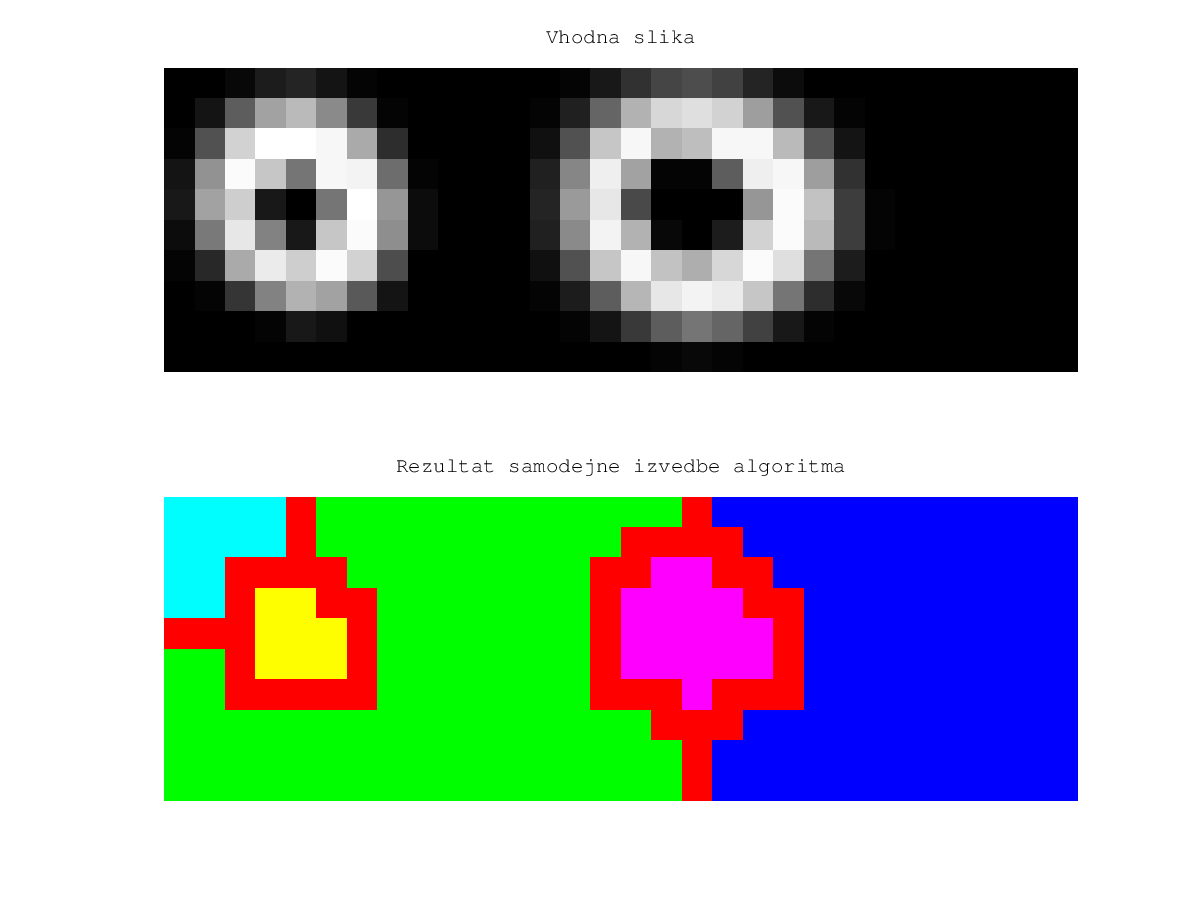
\includegraphics[width=.8\textwidth]{t2-result}
  \caption{Prikaz algoritma na dveh obročih.}
  \label{img:t2-result}
\end{figure}

Na naslednjih treh primerihh pa lahko primerjamo rezultate, ki jih dobimo s samodejno in vodeno različico algoritma. Slika~\ref{img:t4-result} je rezultat samodejnega algoritma, slika~\ref{img:t4-seed-1-result} prikazuje rezultat vodene segmentacije v dve komponenti, slika~\ref{img:t4-seed-2-result} pa ponovno prikazuje vodemo segmentaijo, a z drugačnima semenoma.

\begin{figure}
  \centering
  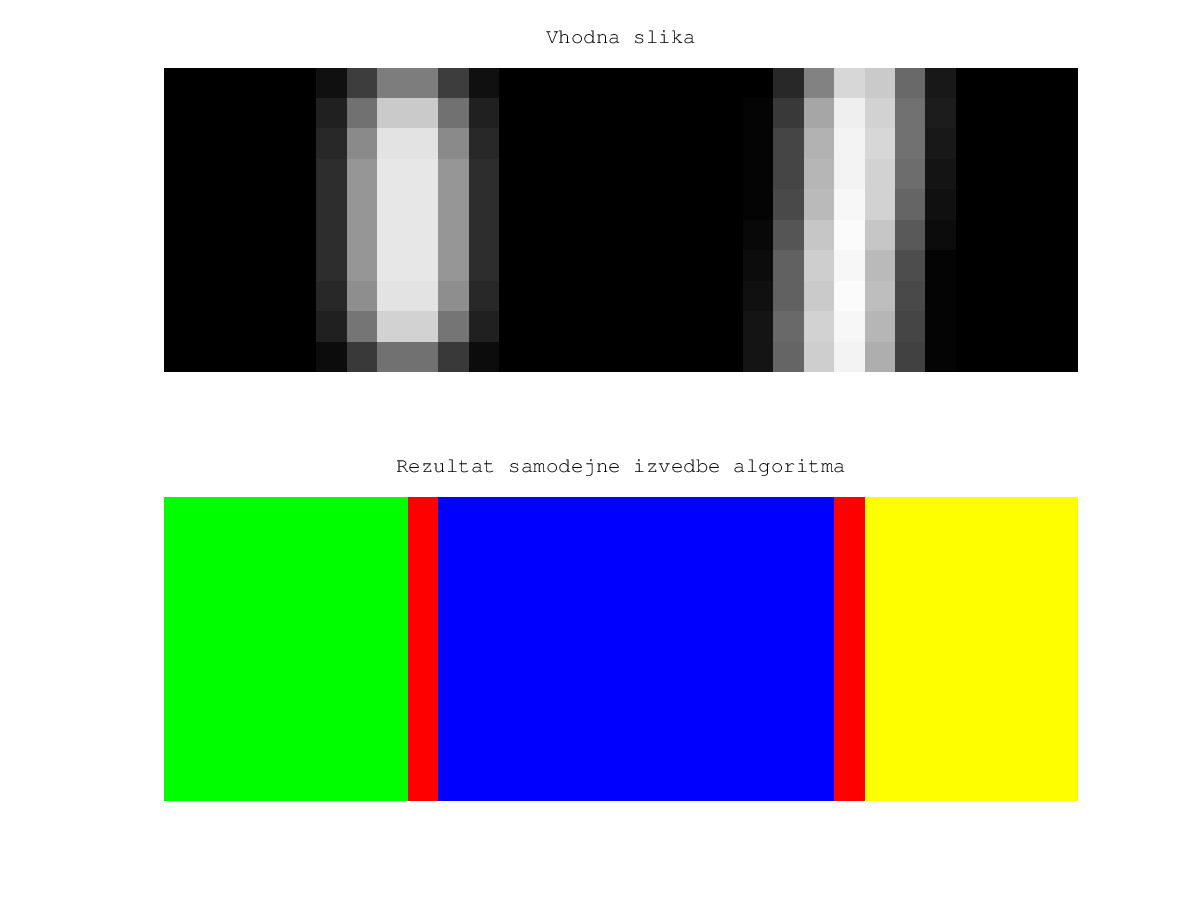
\includegraphics[width=.8\textwidth]{t4-result}
  \caption{Samodejni algoritem na treh prekatih.}
  \label{img:t4-result}
\end{figure}

\begin{figure}
  \centering
  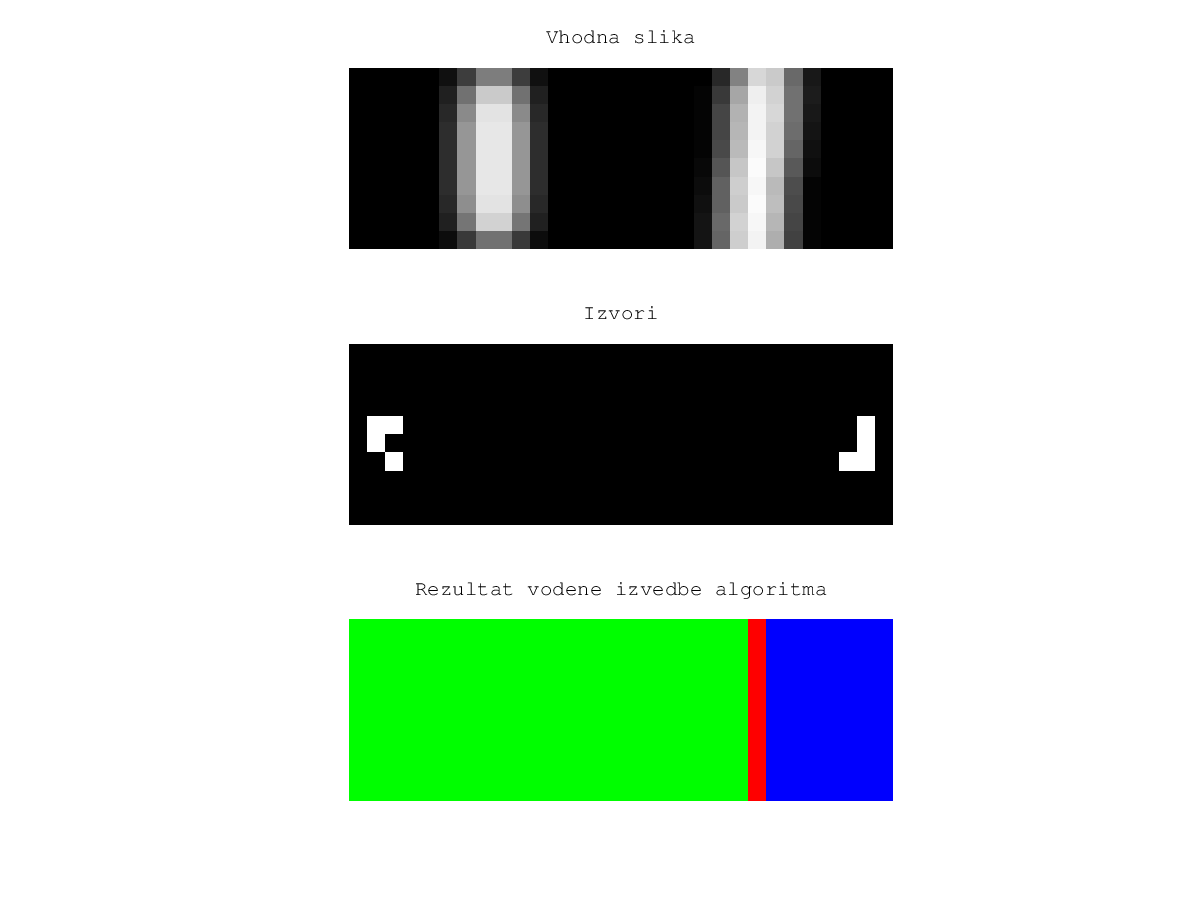
\includegraphics[width=.8\textwidth]{t4-seed-1-result}
  \caption{Vodeni algoritem na treh prekatih.}
  \label{img:t4-seed-1-result}
\end{figure}

\begin{figure}
  \centering
  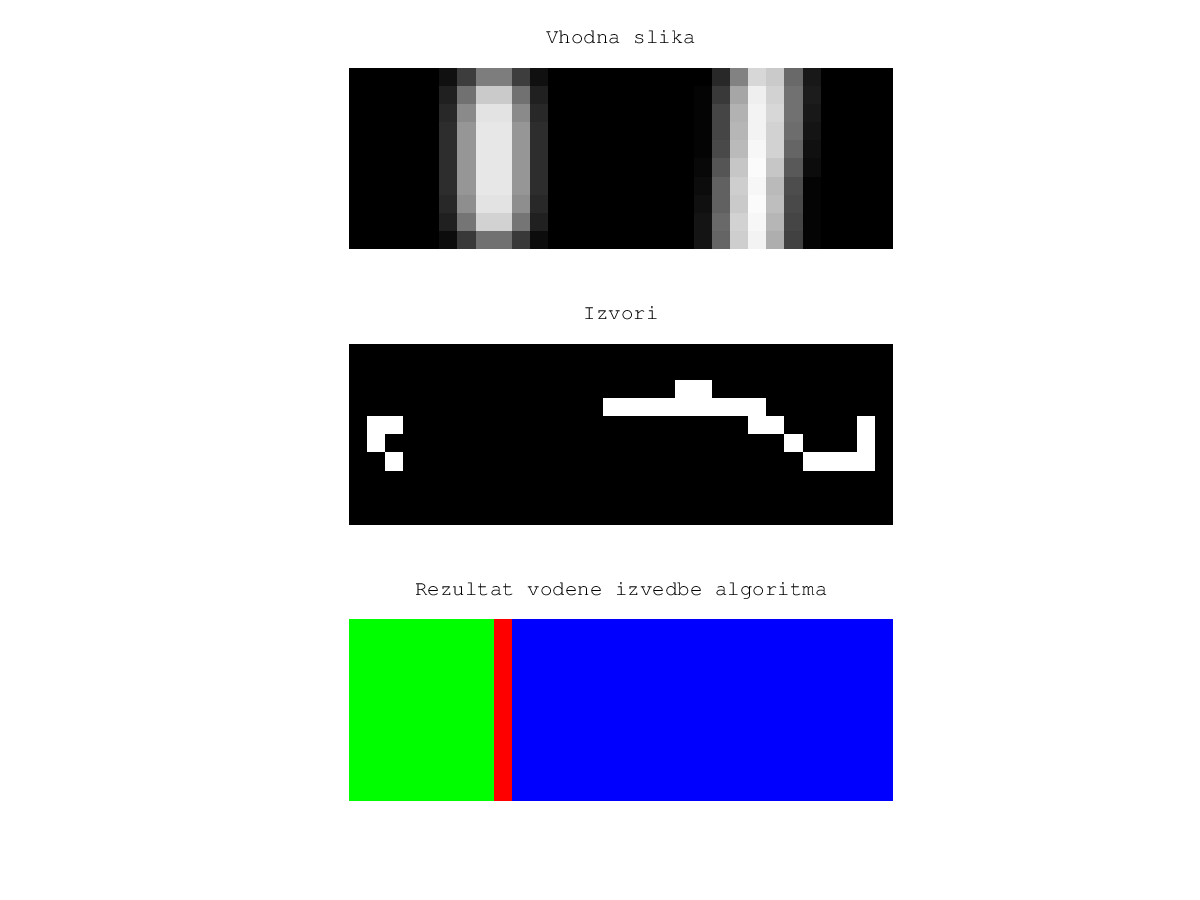
\includegraphics[width=.8\textwidth]{t4-seed-2-result}
  \caption{Vodeni algoritem na treh prekatih.}
  \label{img:t4-seed-2-result}
\end{figure}


\section{Praktični primer}

Kot obljubljeno si bomo sedaj na kratko ogledali enega izmed mogočih načinov uporabe algoritma. V našem primeru bomo skušali poiskati ter osamiti posamezne kovance s slike~\ref{img:coins-input}.

Skozi praktični primer se bomo sprehodili le ob slikah vmesnih rezultatov, izvorna koda programa, ki je pripravil slike, pa je na voljo na \url{https://github.com/tadeboro/dps-sem}.

\begin{figure}[htb]
  \centering
  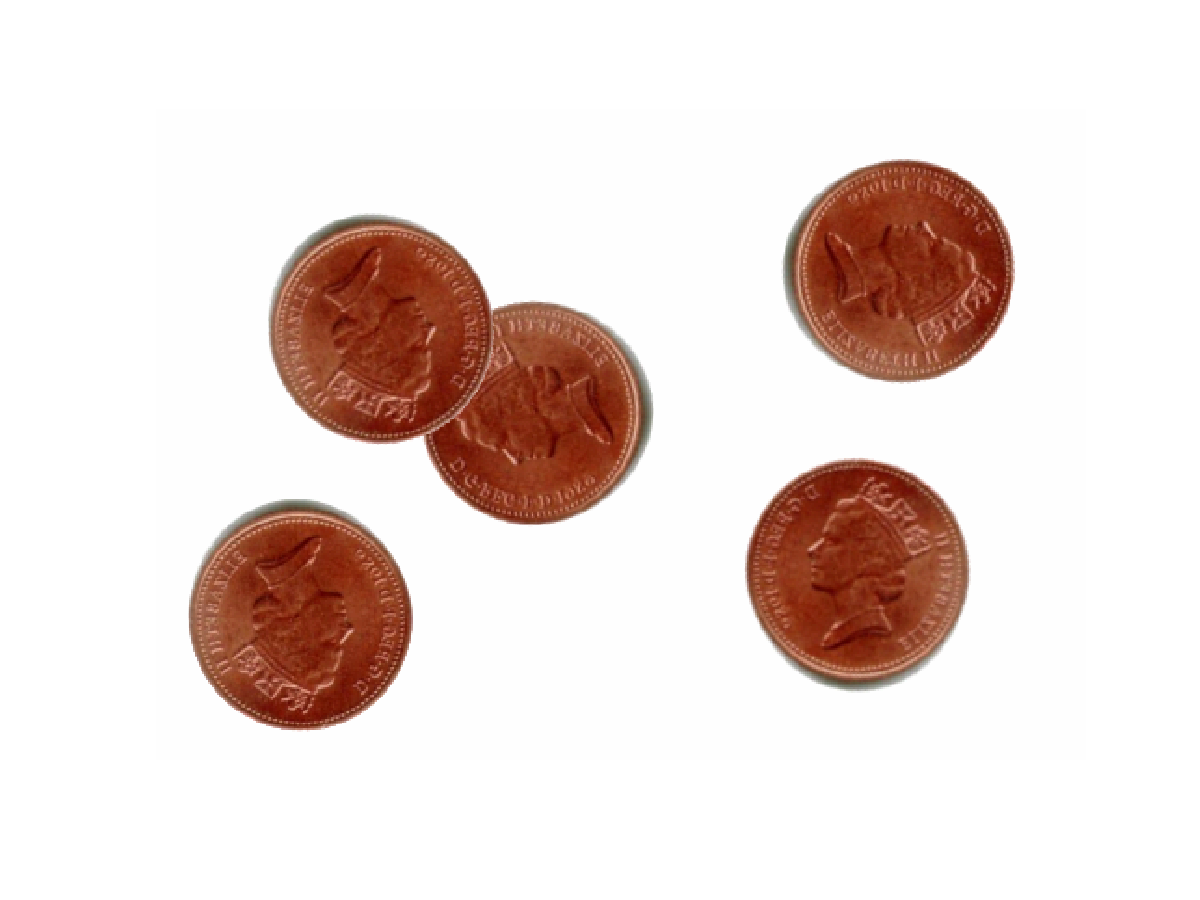
\includegraphics[width=.6\textwidth]{coins-input}
  \caption{Vzorčna slika, s katere želimo izolirati kovance.}
  \label{img:coins-input}
\end{figure}

Na prvem koraku sliki najprej odstranimo ozadje, rezultat odstranitve je prikazan na sliki~\ref{img:coins-bg-rem}. Nato izračunamo oddaljenost vsakega črnega piksla do najbližjega belega in dobimo sliko~\ref{img:coins-distance} (svetlejši deli slike so bolj oddaljeni od črnih ikslov v izvoru). Po filtriranju glede na razdaljo na sliki~\ref{img:coins-seeds} dobimo z belo barvo označene izhodiščne vire za algoritem. Končni rezultat je prikazan na sliki~\ref{img:coins-watershed}.

\begin{figure}[htb]
  \centering
  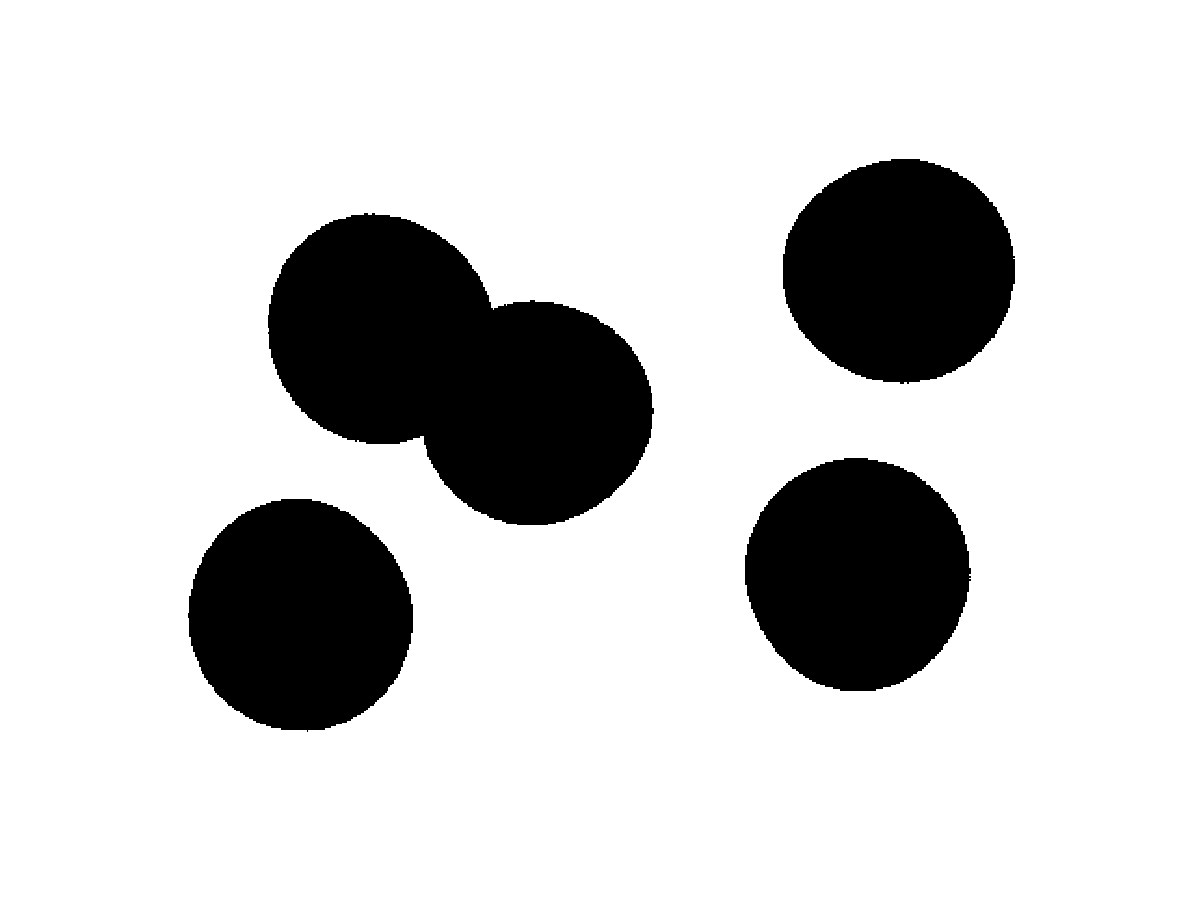
\includegraphics[width=.5\textwidth]{coins-bg-rem}
  \caption{Odstranjeno ozadje.}
  \label{img:coins-bg-rem}
\end{figure}

\begin{figure}[htb]
  \centering
  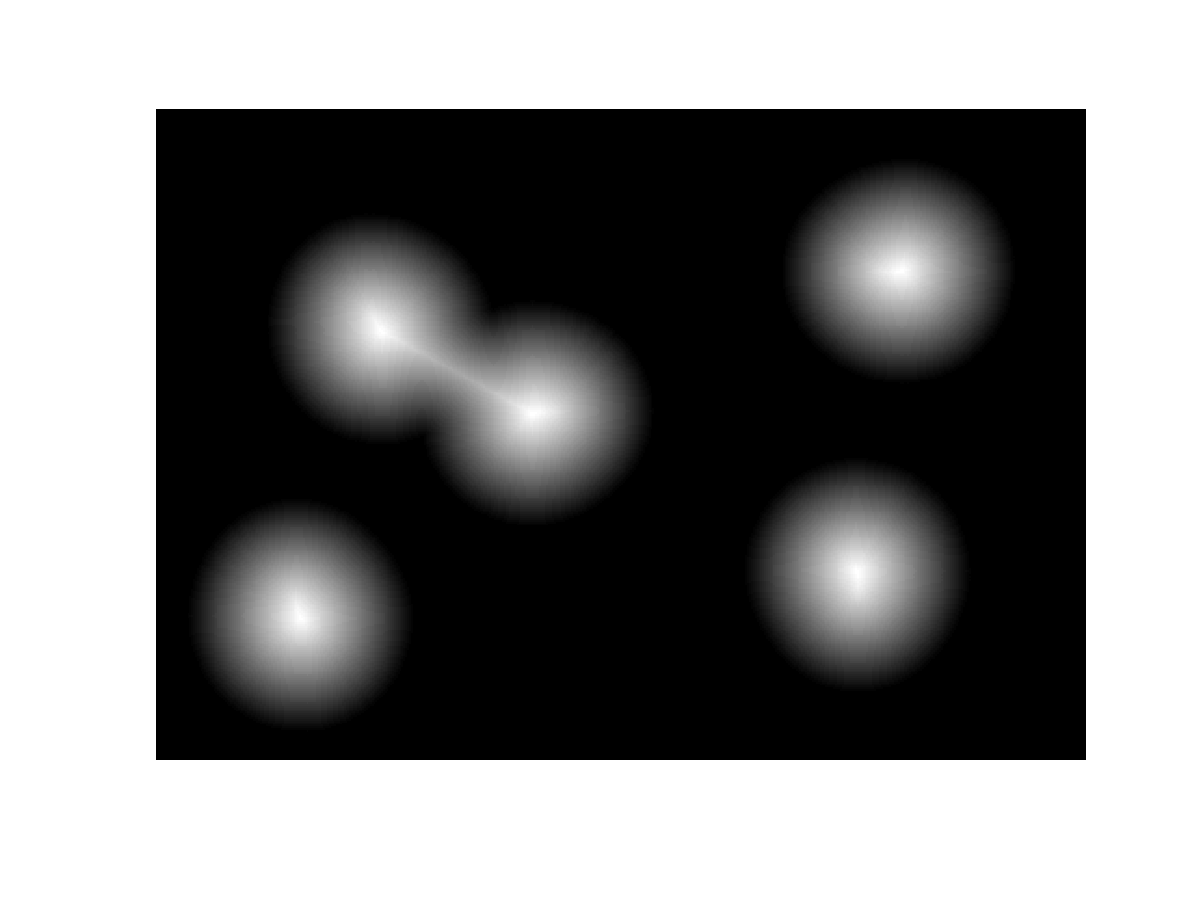
\includegraphics[width=.5\textwidth]{coins-distance}
  \caption{Izmerjene razdalje do ozadja.}
  \label{img:coins-distance}
\end{figure}

\begin{figure}[htb]
  \centering
  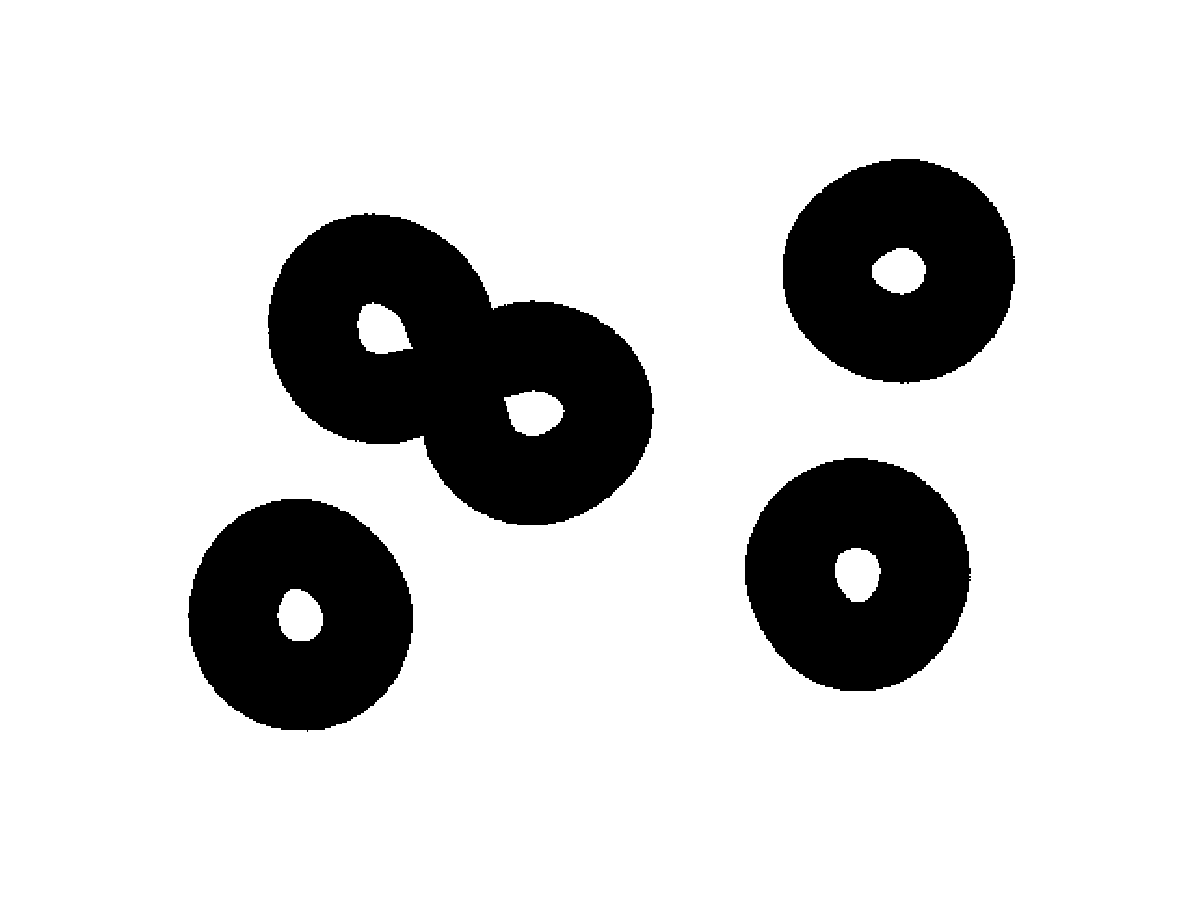
\includegraphics[width=.5\textwidth]{coins-seeds}
  \caption{Začetni izvori.}
  \label{img:coins-seeds}
\end{figure}

\begin{figure}[htb]
  \centering
  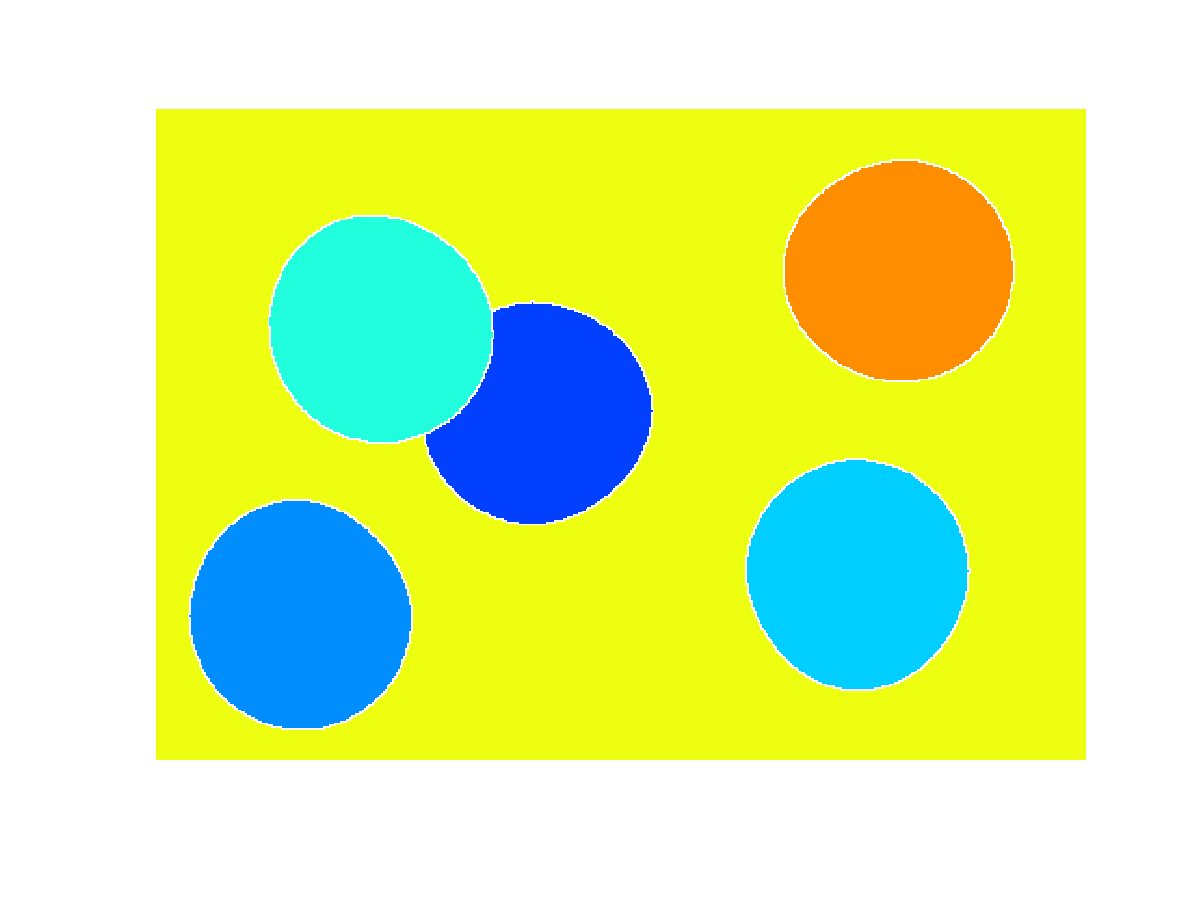
\includegraphics[width=.5\textwidth]{coins-watershed}
  \caption{Segmentirana slika.}
  \label{img:coins-watershed}
\end{figure}

Za ločitev kovancev na sliki v več slik pa sedaj izvedemo maskiranje in obrezovanje vhodne slike s pomočjo maske, ki jo ustvarimo za vsak segment posebej.

Zakaj smo v tem primeru sploh potrebovali algoritem poplavljanja? Težava sta kovanca, ki se prekrivata in pri uporabi večine filtrov tvorita celoto, ki se je ne da enostavno ločiti. Segmentacija s pomočjo vodenega poplavljanja pa nam je omogočila ločiti tudi ta dva kovanca.


\section{Zaključek}

V tem delu smo se precej nežno dotaknili procesiranja slik ter si privoščili kratek izlet v malo manj poznane predele programskega paketa Octave. Pripravili smo ne povsem naivno implementacijo algoritma ter jo uspešno uporabili na praktičnem primeru.

\end{document}
